% SW design
\clearpage

\section{Software design}

Herunder er de forskellige dele af softwaren kort beskrevet. 

\subsection{PC delen (JC)}

Softwaren til PC'en, er brugeren grænseflade til at kontrollere systemet. Her kan han manurære rundt i de forskellige menuer og udføre de forskellige ting som er beskrevet i use casene.

Nedenfor er der illustreret hvordan man kommer frem og tilbage i brugerinterfacet. Udover bruger input så kan CSS hovedenheden give PC'en besked om at der ikke længere er logget ind hvilket vil sende brugeren fra main menu og tilbage til pre-login menuen.

\begin{figure}[htbp] \centering
{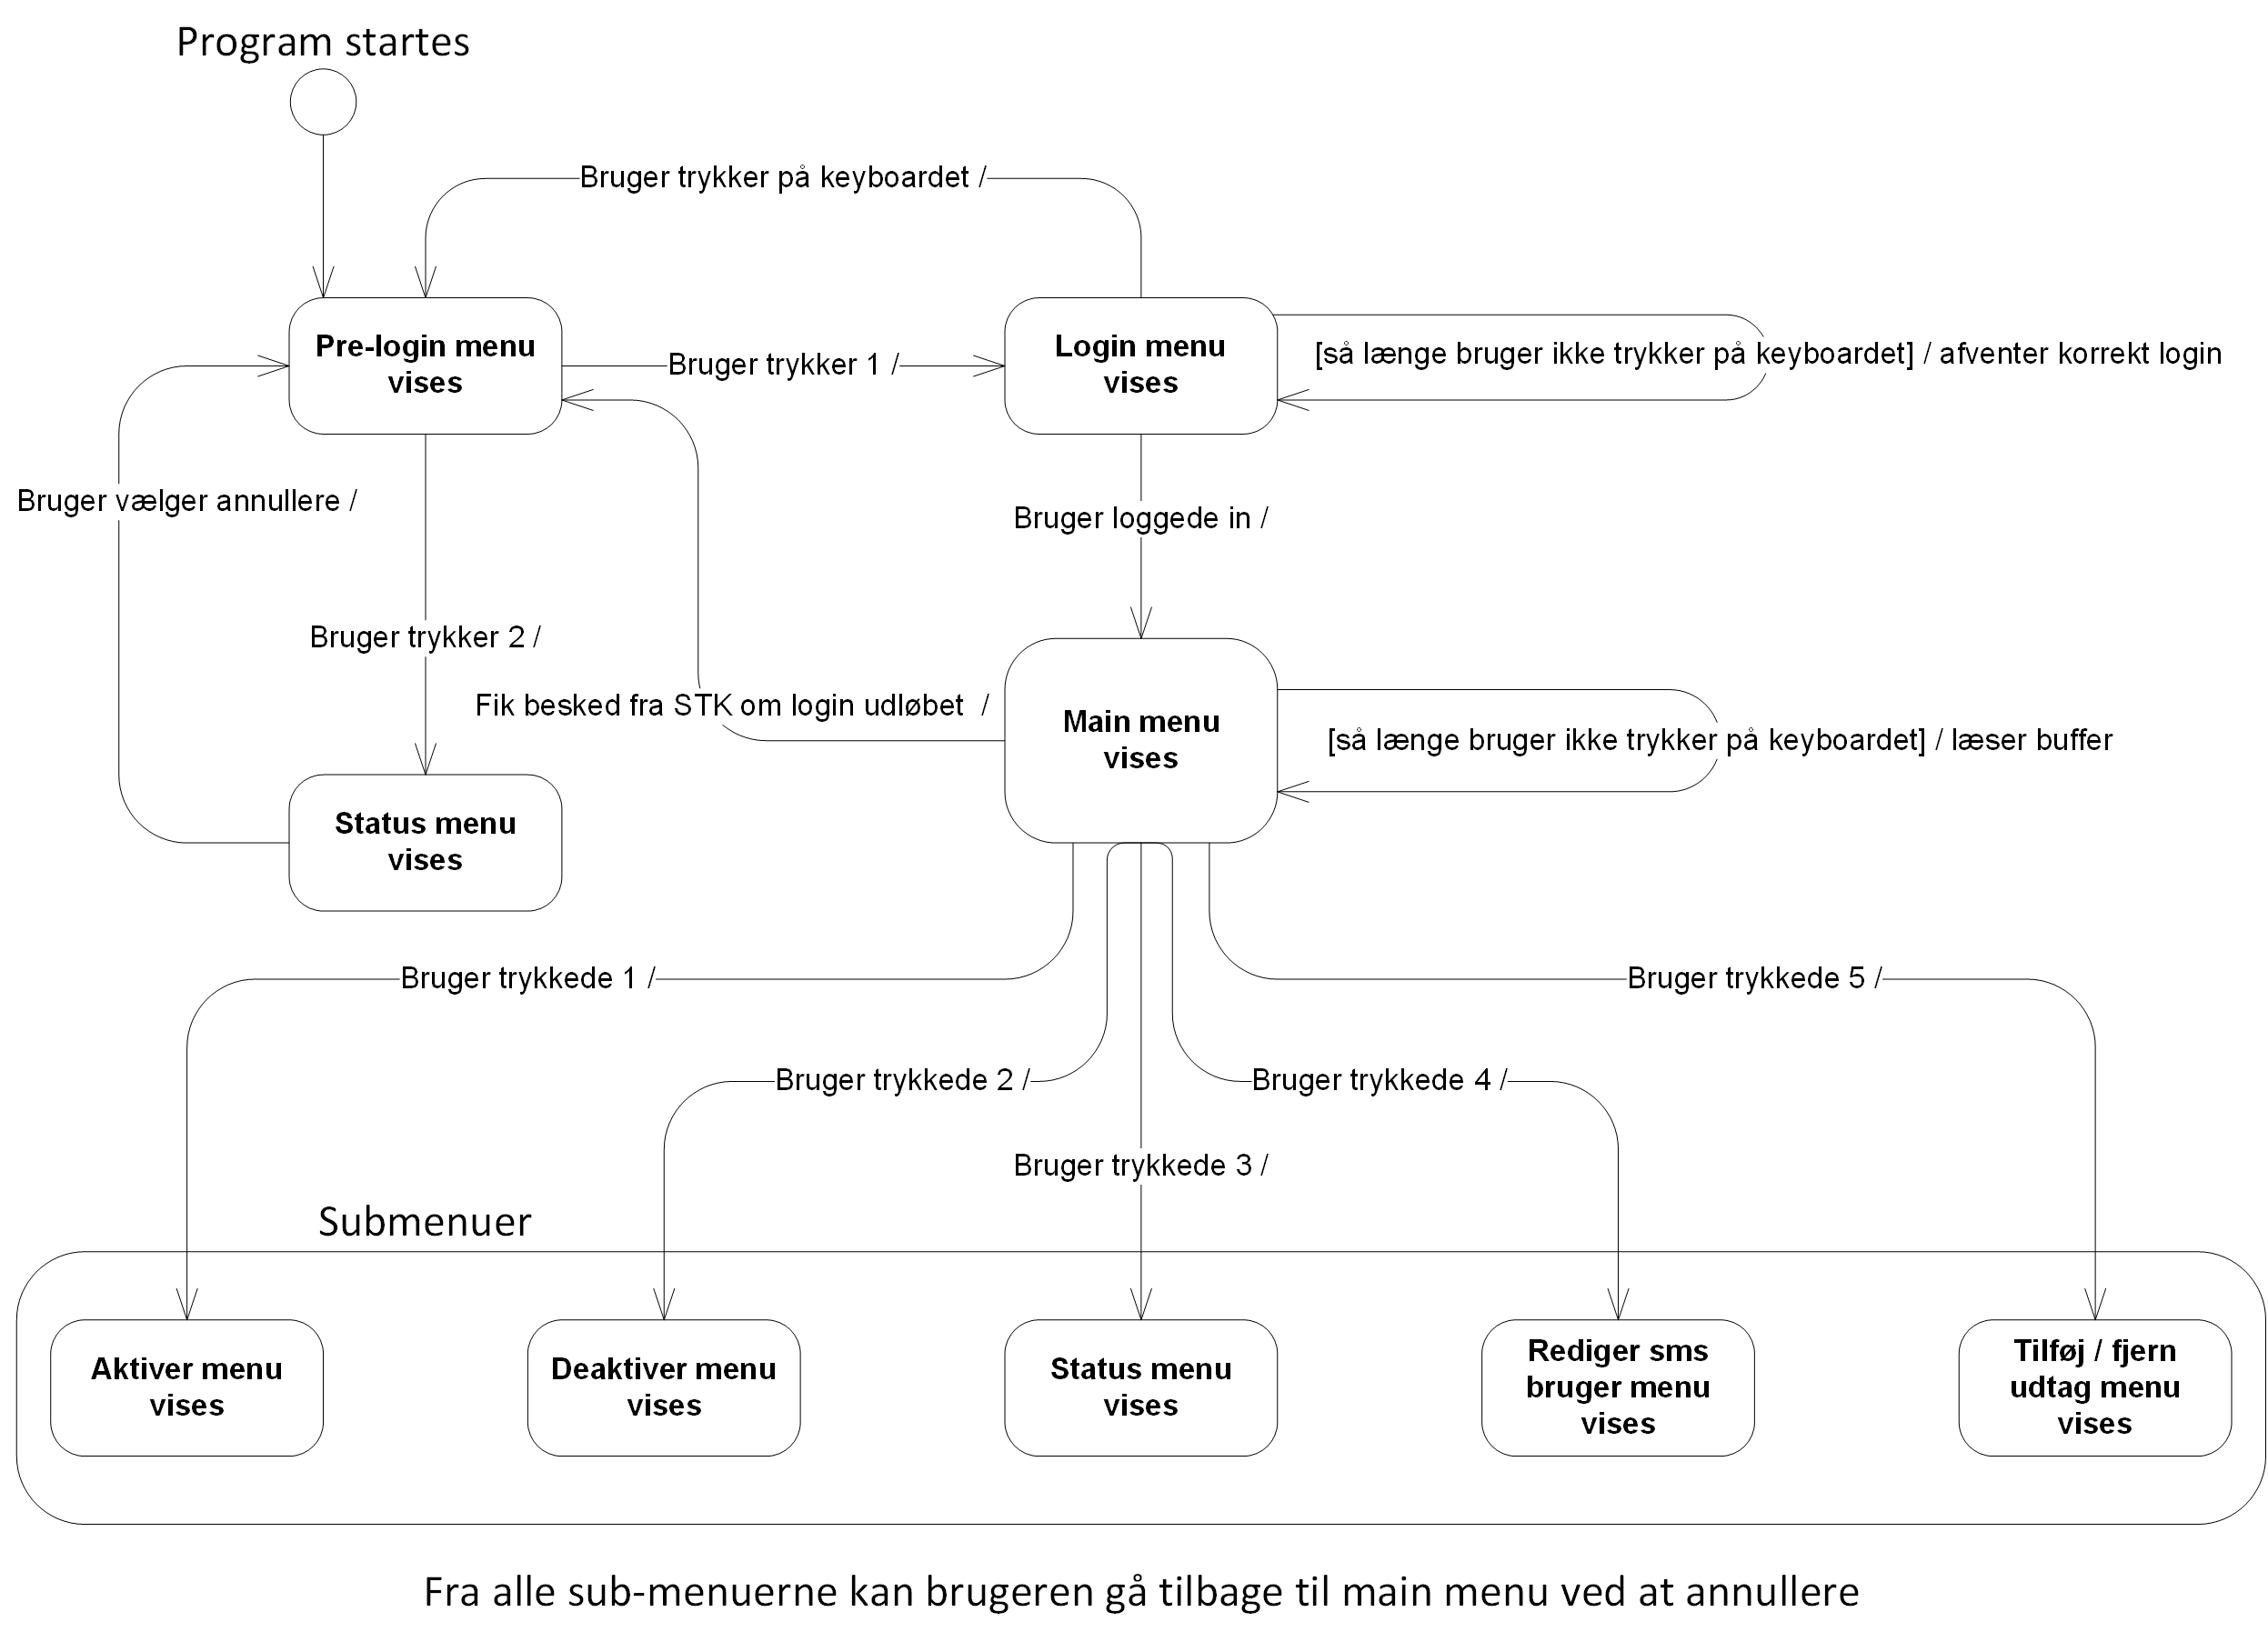
\includegraphics[width=\textwidth]{billeder/uml/state_machine_main}}
\caption{State machine diagram over brugerflade}
\label{lab:State machine diagram over brugerflade}
\end{figure}